\documentclass[12pt,a4paper]{report}

\usepackage[a4paper,margin=1in]{geometry}
\usepackage[T1]{fontenc}
\usepackage[utf8]{inputenc}
\usepackage{newtxtext,newtxmath}
\usepackage{setspace}
\usepackage{graphicx}
\graphicspath{{figures/}}
\usepackage{booktabs}
\usepackage{array}
\usepackage{longtable}
\usepackage{tabularx}
\usepackage{float}
\usepackage{caption}
\usepackage{subcaption}
\usepackage{amsmath}
\usepackage{enumitem}
\usepackage{titlesec}
\usepackage{fancyhdr}
\usepackage{hyperref}
\usepackage{url}
\usepackage{cite}
\usepackage{xcolor}
\usepackage{listings}

\hypersetup{
    colorlinks=true,
    linkcolor=black,
    citecolor=black,
    urlcolor=blue
}

\setlength{\parindent}{0.5in}
\setlength{\parskip}{0pt}
\onehalfspacing

\titleformat{\chapter}[display]
{\bfseries\centering\Large}
{Chapter \thechapter}
{0.5em}
{\Large}

\titleformat{\section}
{\bfseries\normalsize}
{\thesection}
{0.75em}
{}

\titleformat{\subsection}
{\bfseries\normalsize}
{\thesubsection}
{0.75em}
{}

\pagestyle{fancy}
\fancyhf{}
\fancyhead[R]{\thepage}
\renewcommand{\headrulewidth}{0pt}

\lstset{
    language=Python,
    basicstyle=\ttfamily\small,
    breaklines=true,
    frame=single,
    columns=fullflexible,
    keepspaces=true,
    showstringspaces=false
}

\begin{document}

\begin{titlepage}
    \thispagestyle{empty}
    \begin{center}
        \vspace*{0.8cm}
        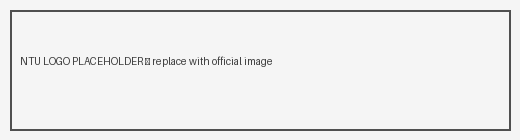
\includegraphics[width=0.5\linewidth]{ntu_logo.png}\\[3.2cm]
        {\large PCCDS24-0086\par}
        \vspace{0.35cm}
        {\bfseries
        \large Scenario Generation Methods for Functional Safety Testing Of Automated Driving Systems\par}
        \vspace{1.4cm}
        {\large Submitted by: Chaw Kay Khine\par}
        \vspace{2.3cm}
        {\normalsize Supervisor: Prof Liu Yang\par}
        \vspace{0.25cm}
        {\normalsize Co-supervisor: Wen Bing\par}
        \vspace{1.8cm}
        {\normalsize School of Computer Science and Engineering\par}
        \vspace{1.6cm}
        {\normalsize A final year project report presented to Nanyang Technological University\par}
        \vspace{0.2cm}
        {\normalsize in partial fulfilment of the requirements for the\par}
        \vspace{0.2cm}
        {\normalsize Degree of Bachelor of Engineering\par}
        \vfill
        {\normalsize 2024/2026\par}
    \end{center}
\end{titlepage}

\pagenumbering{roman}

\chapter*{Abstract}
Automated driving systems must be shown to behave safely enough for their intended use. Scenario-based testing supports this goal by exercising the system under controlled conditions that resemble real traffic. Examples include routine urban driving, congested traffic, and more demanding situations, without putting road users at avoidable risk. High-fidelity three-dimensional simulators help because traffic, road layout, and events can be changed in a controlled and repeatable way.

Even with simulation, the set of possible situations is huge. It is not feasible to run every combination. Test design therefore needs ways to select or generate scenarios that matter for functional safety, give enough diversity to cover important behaviours, and avoid unnecessary repetition. Finding critical scenarios that stress the system and reveal weaknesses, while keeping the test campaign efficient, is an active line of work in research and industry.

This project is carried out in Desay's context. It reviews and applies state-of-the-art scenario-based testing methods in simulation, evaluates how well they fit this setting, and identifies limitations when those methods are checked against Desay's requirements. Building on that review, the work explores directions for more efficient generation of critical scenarios, with emphasis on useful coverage rather than purely random sampling.

This report therefore links general ideas in scenario-based safety evaluation to a concrete industrial framing. It presents the methodology, evaluation, and findings on that basis, and states openly what is left for future work.

\vspace{0.5em}
\noindent\textbf{Keywords:} automated driving systems, functional safety, scenario-based testing, scenario generation, critical scenarios, simulation, diversity, redundancy.

\tableofcontents
\listoffigures
\listoftables

\clearpage
\pagenumbering{arabic}

\chapter{Introduction}

\section{Background and Motivation}
Automated driving systems are expected to support real traffic with an acceptable level of risk. Showing that level in a convincing way is often grouped under functional safety and related testing practice \cite{iso26262,iso21448,sae3016}. Because public-road experiments are costly, slow, and constrained by safety and regulation, simulation is a standard step. High-fidelity three-dimensional simulators allow traffic, geometry, and events to be varied in a controlled way while keeping tests repeatable and measurable \cite{pegasus_method,carla_official,metadrive_docs}.

Scenario-based testing is a common way to use that capability. Instead of hoping that a long random drive will expose every important failure mode, engineers define situations the system should survive or handle well. These can range from routine urban driving and congested conditions to more demanding cases that stress perception, prediction, or control. The approach is widely discussed in research and industry, and it is not introduced here as a new invention. It is used because it matches how automated driving systems are actually questioned in development and audit-style discussions \cite{openscenario_standard,pegasus_method}.

The practical difficulty is scale. Even inside one simulator, the combination of maps, actors, timings, and disturbances grows very quickly. It is not possible to execute every combination. Test design therefore turns into a search problem in a very large space. Practitioners need sets of scenarios that are relevant for safety, diverse enough to cover different mechanisms of failure, and not full of near-duplicates that waste computation and review time.

This report is placed in Desay's context. The aim is not to restate general theory only, but to connect published state-of-the-art ideas in scenario-based testing to requirements and constraints that matter for that setting.

\section{Problem Statement}
Scenario-based testing is a standard way to check automated driving systems in simulation, but the space of possible situations is very large. A practical risk is that tests repeat similar cases, miss important failures, or produce a pass rate that looks acceptable until timeouts, contacts, and finish times are inspected separately. For a safety-oriented discussion, the problem is to define logging and metrics that show how a run failed, not only whether it was marked as a pass.

When the same kind of controller is run under different road contexts, such as highway-style flow versus intersection-style crossing, recorded outcomes can change strongly. A single blended score or a short informal demonstration can then hide the main failure mode or give a misleading ranking between policies.

\section{Aim and Objectives}
\subsection*{Aim}
The aim of this report is to support functional-safety-oriented discussion for automated driving by using scenario-based tests in simulation, and by studying how outcomes change with scenario context and with the way results are measured.

\subsection*{Objectives}
The main objective of this project is to develop, implement, and assess an autonomous driving simulation framework in MetaDrive for comparative evaluation of driving policies under different road scenarios, including highway, intersection, and street settings.

\vspace{0.5em}
The specific objectives are:
\begin{enumerate}[label=\arabic*.]
    \item To create and configure three representative simulation scenarios covering different categories of road interaction.
    \item To implement and test several driving policies.
    \item To introduce scenario-specific mechanisms where necessary, such as fixed-route multi-agent behaviour and pedestrian-crossing events.
    \item To collect and export data from repeated simulation episodes for analysis.
    \item To evaluate and compare policy performance using measures such as completion rate, timeout rate, crash frequency, speed, and travel time.
    \item To identify the most appropriate policy for each scenario based on the experimental results.
\end{enumerate}

\section{Research Evolution}
The evolution of the experimental platform reflects a structured evaluation of simulation tools against the project requirements and resource constraints. Initially, no single simulator was prescribed. The first implementation centred on SUMO for mixed-traffic analysis \cite{sumo,treiber2000congested,sumo_docs}. As the emphasis shifted toward functional-safety-oriented testing, limitations became evident, including limited three-dimensional visualisation for documentation and review, restricted flexibility for generating diverse safety-critical situations, and the absence of an integrated safety test workflow without substantial additional development.

\begin{figure}[H]
    \centering
    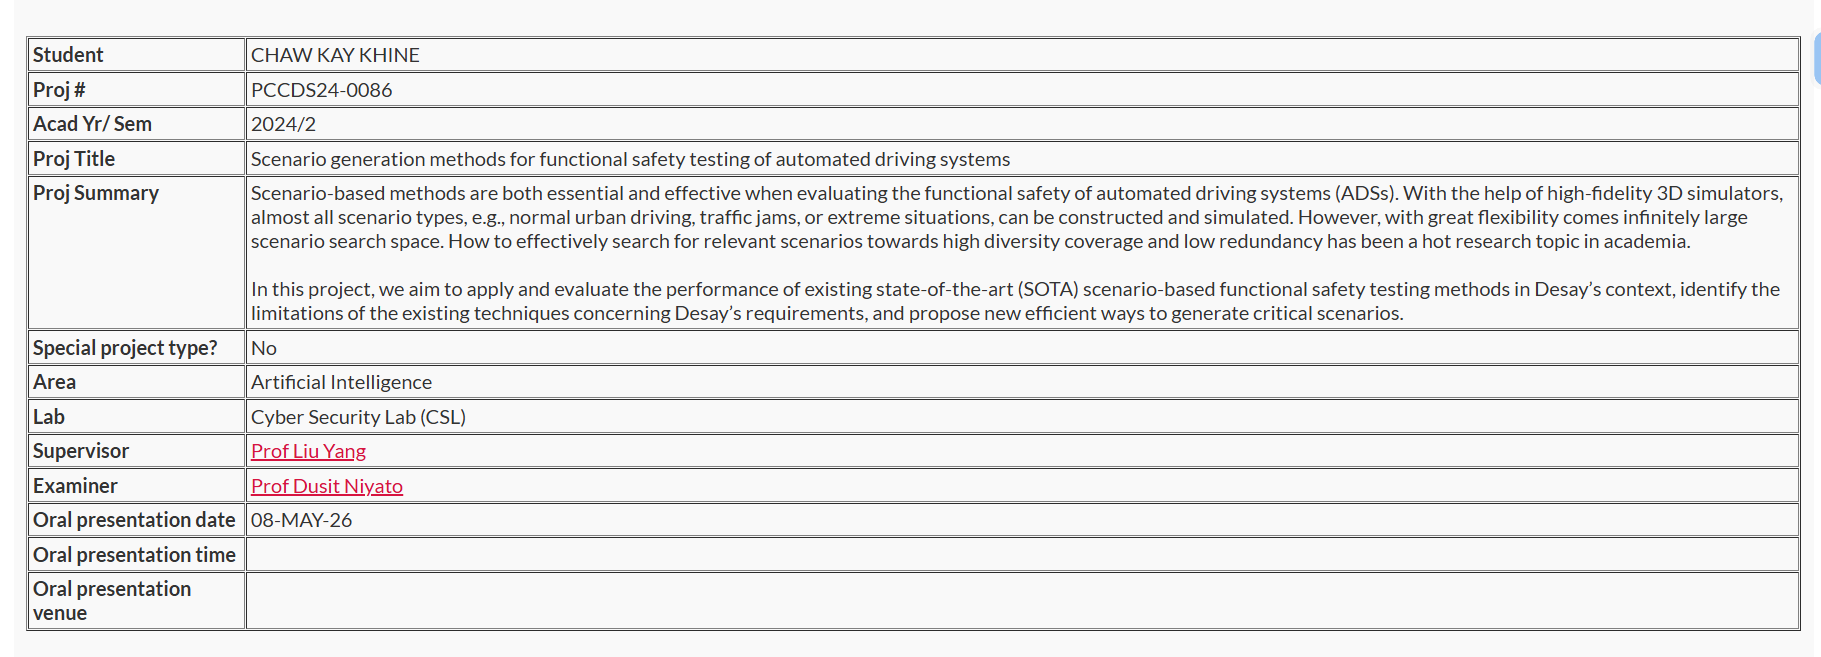
\includegraphics[width=0.8\textwidth]{fyp_description.png}
    \caption{Initial platform limitations and project framing.}
    \label{fig:fyp_description}
\end{figure}

Subsequently, CARLA was evaluated as a candidate platform owing to its high-fidelity environments and its alignment with sensor-based pipelines commonly reported in the literature \cite{carla,carla_official}. The project therefore standardised on MetaDrive \cite{metadrive,metadrive_docs}, which provided compositional scenario generation, three-dimensional visualisation suitable for reporting, and iteration times compatible with batched experiments under the available hardware and access arrangements.

\section{Report Structure}
Chapter 2 reviews background literature and concepts related to autonomous driving evaluation, functional safety, and scenario generation.

Chapter 3 describes the methodology, including simulator selection, scenarios, policies, experimental procedure, and metric definitions.

Chapter 4 presents the system design of the evaluation framework at an architectural level.

Chapter 5 documents the implementation in detail, including representative code, the experimental procedure, and parameter settings.

Chapter 6 presents the results, notebook-based visual analysis, and discussion.

Chapter 7 concludes the report and outlines future work.

\chapter{Literature Review}

\section{Automated Driving System Testing}
Road testing gives realism but scales poorly for rare or hazardous situations. Simulation is widely used to add repeatability, volume, and access to cases that would be hard to stage on the road. Scenario-based testing means exercising the system through defined situations rather than one undifferentiated long drive \cite{pegasus_method,openscenario_standard}.

\section{Functional Safety Standards}
ISO 26262 is commonly used when discussing functional safety processes for road vehicles, including hazard analysis and structured verification and validation \cite{iso26262}. ISO 21448 draws attention to risk that arises when the system behaves as intended but still fails to handle the world correctly \cite{iso21448}. SAE J3016 supplies shared definitions for automation levels and related terms \cite{sae3016}.

\section{Scenario Generation Methods}
Rule-based methods encode constraints from regulations and engineering judgement. Data-driven methods build scenarios from recorded driving. Search-based methods optimise scenario parameters to stress the system. Compositional methods combine smaller elements into full scenarios \cite{pegasus_method,openscenario_standard}. The project does not require choosing one family forever; it requires a method that matches the tool, the time limit, and the evidence the report must show.

\section{Simulation Platform Analysis}
Various simulation platforms have been developed for automated driving research, each offering different capabilities and trade-offs. CARLA provides realistic urban environments with high-fidelity graphics and comprehensive sensor simulation but requires significant computational resources \cite{carla,carla_official}. SUMO specialises in large-scale traffic simulation but lacks three-dimensional visualisation and advanced physics simulation \cite{sumo,sumo_docs}. MetaDrive distinguishes itself through its focus on AI and autonomy research, offering compositional scenario generation, realistic physics simulation, lightweight design, and comprehensive safety testing features \cite{metadrive,metadrive_docs}.

\begin{figure}[H]
    \centering
    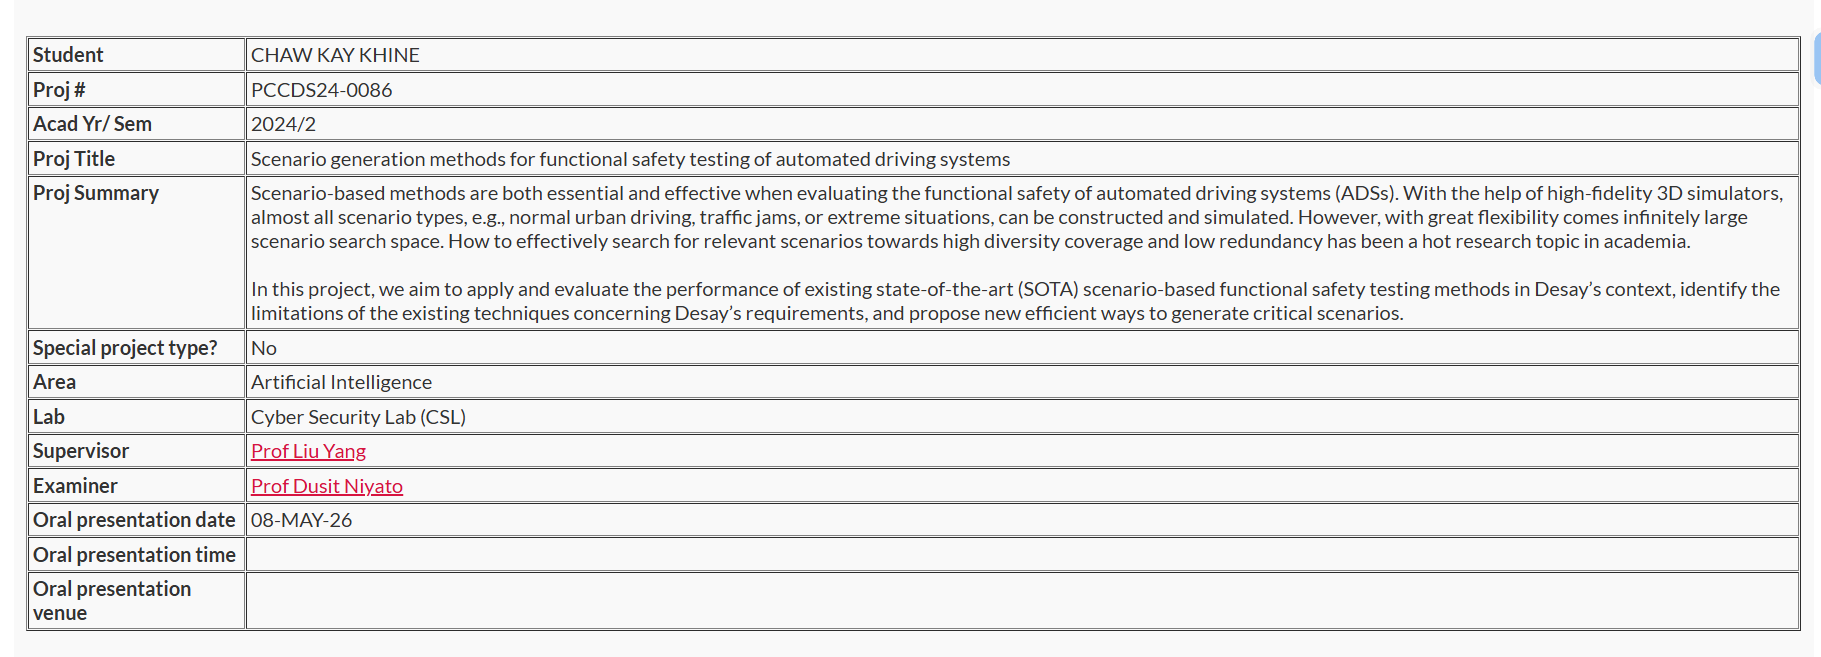
\includegraphics[width=0.78\textwidth]{fyp_description.png}
    \caption{CARLA figure placeholder. Replace with the intended CARLA image in Overleaf if needed.}
    \label{fig:carla_placeholder}
\end{figure}

\begin{figure}[H]
    \centering
    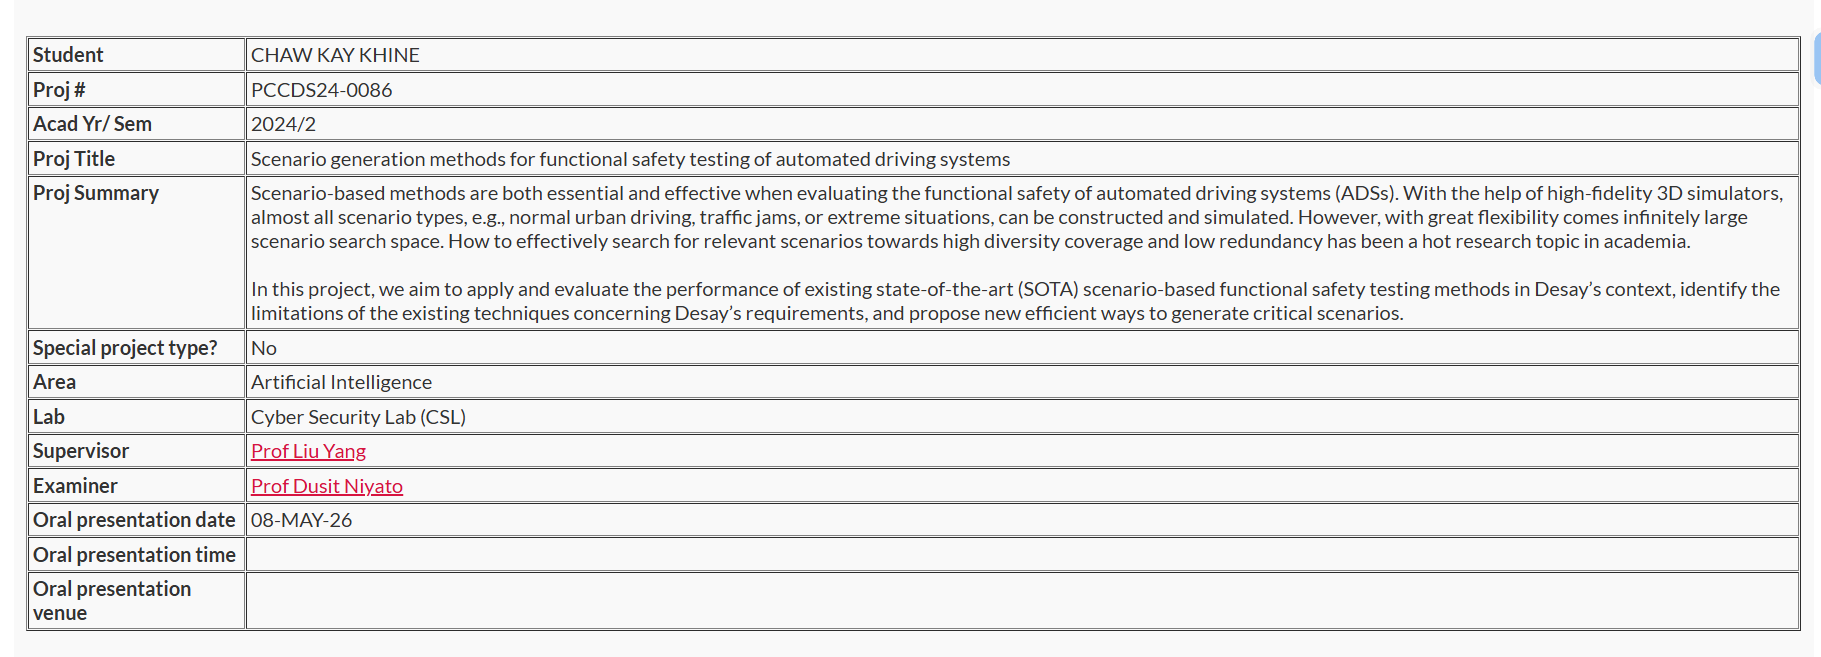
\includegraphics[width=0.78\textwidth]{fyp_description.png}
    \caption{MetaDrive figure placeholder. Replace with the intended MetaDrive image in Overleaf if needed.}
    \label{fig:metadrive_placeholder}
\end{figure}

\chapter{Research Methodology and Platform Selection}

\section{Initial Approach with SUMO}
The research initially employed SUMO as the primary simulation platform for analysing automated vehicle behaviours in mixed traffic environments \cite{sumo,sumo_docs}. The implementation focused on preparation, simulation, and analysis. During preparation, traffic scenarios including lane changes, emergency braking, and intersection navigation were designed. The simulation phase involved implementing automated vehicle features such as adaptive cruise control and executing mixed traffic simulations with data collection on safety, efficiency, and comfort metrics.

\begin{figure}[H]
    \centering
    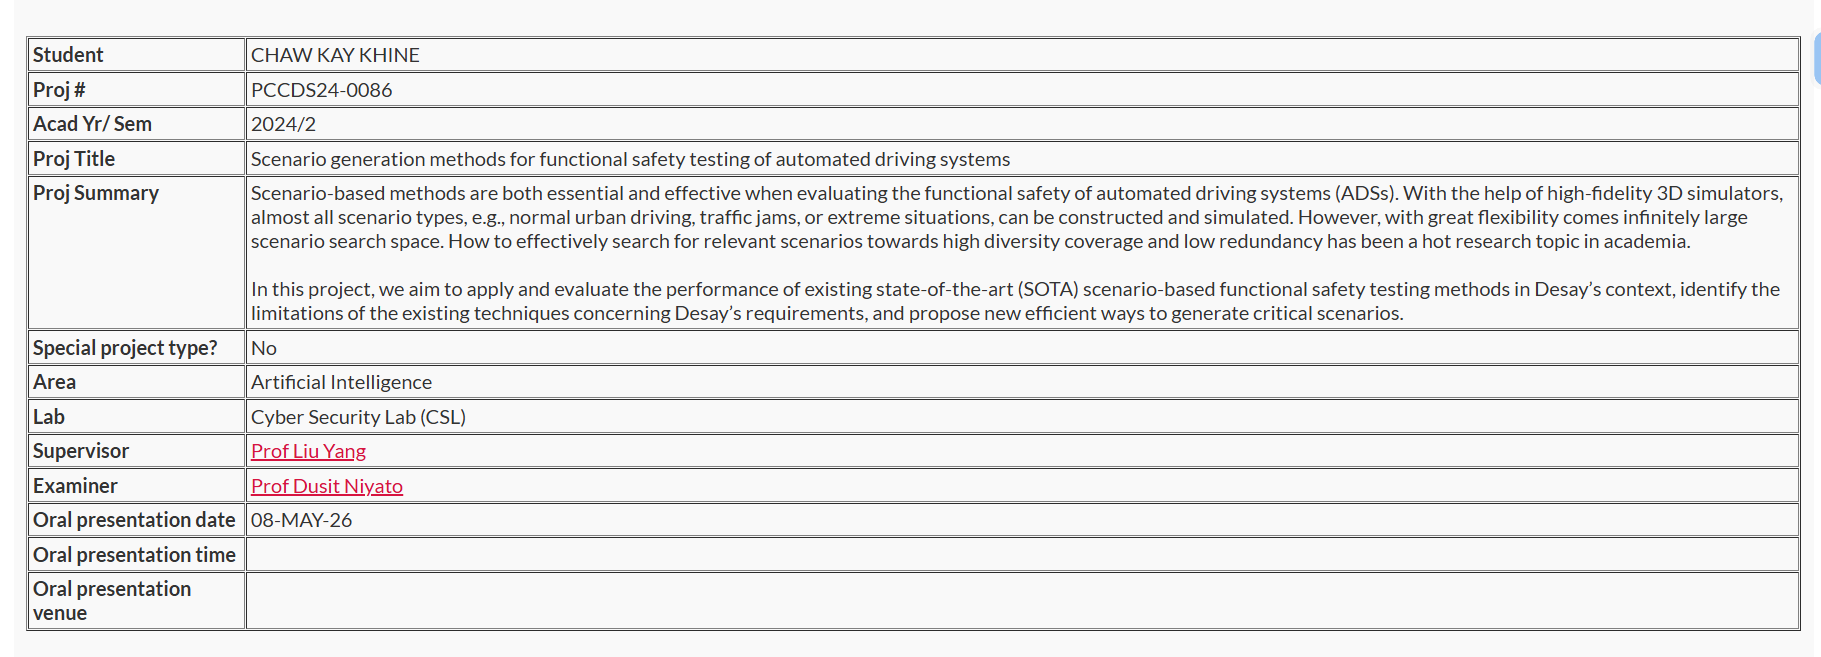
\includegraphics[width=0.75\textwidth]{fyp_description.png}
    \caption{SUMO vehicle analysis placeholder. Replace with the intended figure from the report assets.}
    \label{fig:sumo_analysis}
\end{figure}

\begin{figure}[H]
    \centering
    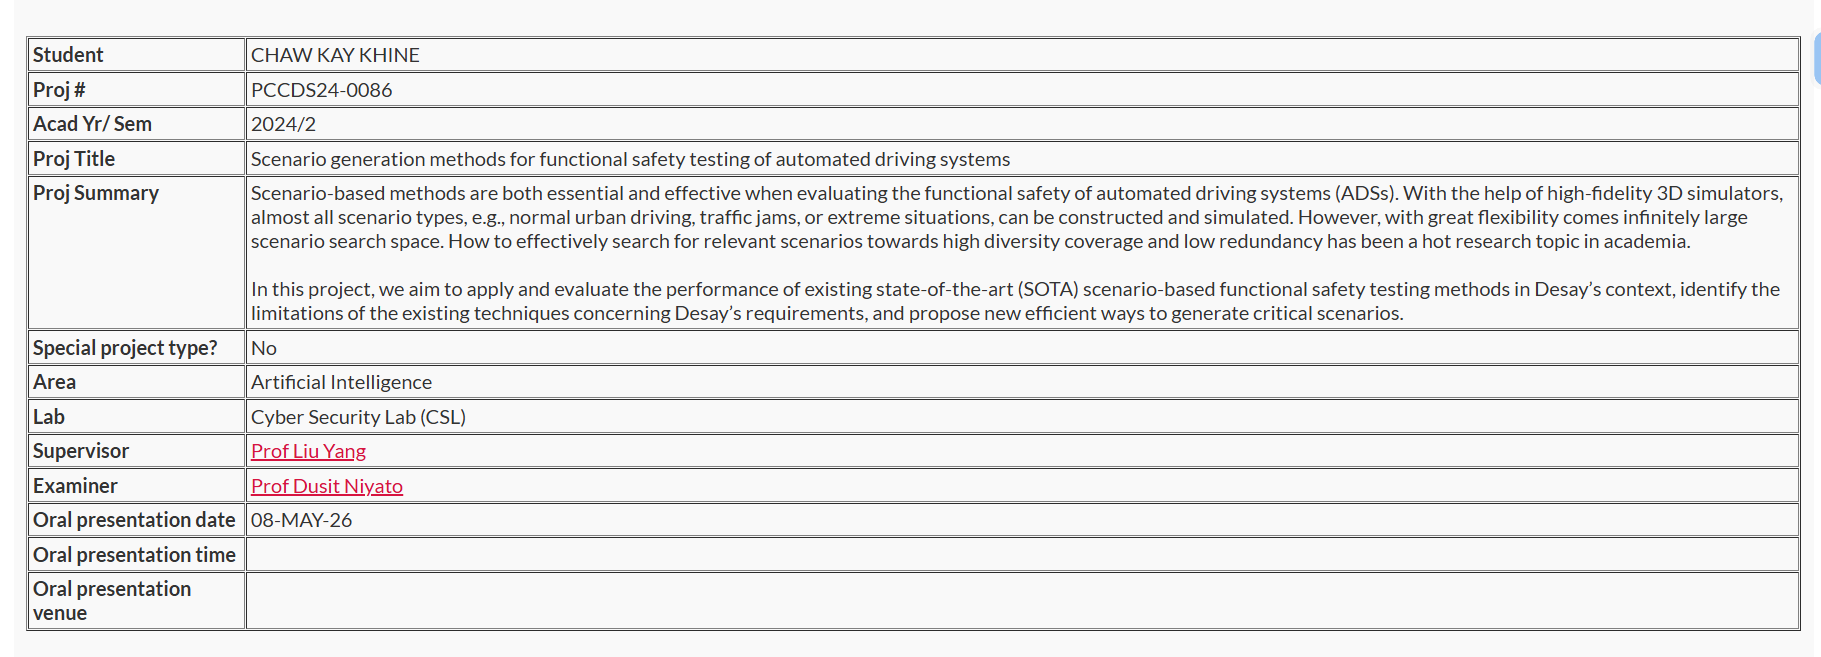
\includegraphics[width=0.75\textwidth]{fyp_description.png}
    \caption{SUMO result visualisation placeholder. Replace with the intended figure from the report assets.}
    \label{fig:sumo_result}
\end{figure}

\section{Platform Evaluation and Transition}
Comprehensive evaluation of SUMO's capabilities for functional safety testing revealed limitations that impacted the research objectives. SUMO's two-dimensional visualisation restricted the ability to create realistic driving scenarios with proper depth perception and spatial awareness. The platform's scenario generation capabilities were limited in terms of diversity and complexity for safety-critical situations. SUMO's simplified physics model did not provide the level of realism required for comprehensive functional safety testing, and it lacked built-in features for systematic safety testing and evaluation \cite{sumo_docs}.

These limitations led to evaluation of alternative platforms, with MetaDrive emerging as the most suitable option due to its focus on AI and autonomy research, comprehensive safety testing features, and scenario generation capabilities \cite{carla_official,metadrive_docs}.

\section{MetaDrive Framework Implementation}
The transition to MetaDrive enabled implementation of a framework for functional safety testing with significantly enhanced capabilities. MetaDrive's compositional scenario generation allows creation of many scenario variations through systematic combination of road configurations, traffic patterns, and environmental conditions. The platform's realistic physics simulation provides accurate vehicle dynamics, collision detection, and environmental interactions essential for reliable safety assessment. MetaDrive's built-in safety testing features, including the \texttt{SafeMetaDriveEnv} environment, offer comprehensive safety monitoring with collision detection, out-of-bounds detection, and related safety metrics \cite{metadrive,metadrive_docs}.

\begin{table}[H]
    \centering
    \caption{MetaDrive Core Architecture Workflow}
    \label{tab:metadrive_workflow}
    \begin{tabularx}{\textwidth}{>{\raggedright\arraybackslash}p{3cm} X}
        \toprule
        Component & Description \\
        \midrule
        Action Input & Policy outputs steering and throttle or control decisions. \\
        Simulation Core & Physics, world state updates, traffic interaction, and route logic are processed. \\
        Sensor Layer & Cameras, LiDAR, and state information are generated from the updated environment. \\
        Output Layer & Observations, rewards, and termination signals are returned for logging and analysis. \\
        \bottomrule
    \end{tabularx}
\end{table}

\begin{table}[H]
    \centering
    \caption{SUMO vs MetaDrive Platform Evaluation}
    \label{tab:sumo_vs_metadrive}
    \begin{tabularx}{\textwidth}{>{\raggedright\arraybackslash}p{3cm} X X}
        \toprule
        Criterion & SUMO & MetaDrive \\
        \midrule
        Visualisation & Mainly two-dimensional & Three-dimensional simulation and rendering \\
        Physics realism & Simplified traffic-oriented dynamics & More suitable for vehicle-level safety experiments \\
        Scenario generation & Good for traffic flow studies & Strong compositional scenario generation \\
        Safety testing support & Requires extra workflow development & Better direct support for episode-level safety evaluation \\
        Iteration speed & Strong for traffic studies & Strong for autonomy-focused simulation under project constraints \\
        \bottomrule
    \end{tabularx}
\end{table}

\chapter{System Design}

This chapter explains \emph{what} the evaluation framework is intended to do and \emph{how} its major pieces fit together. Detailed code listings, file paths, and step-by-step execution logic are deferred to Chapter~5 so that design rationale stays readable on its own.

\section{Purpose and Scope of the Framework}
The framework wraps MetaDrive \cite{metadrive,metadrive_docs} so that multiple driving policies can be compared under fixed scenario definitions. Each run produces structured episode records (pass or fail, timeouts, crashes, timing, speed) that can be aggregated consistently across policies. The scope is deliberately simulation-only: the goal is repeatable comparative evidence, not certification of a production stack.

\section{Layered Architecture}
Figure~\ref{fig:arch_layers} summarises the system as four cooperating layers. The same layering applies to every scenario script, which keeps batch experiments and later analysis predictable.

\begin{enumerate}[label=\textbf{L\arabic*:}, leftmargin=2.2cm]
    \item \textbf{Scenario layer.} Chooses map topology, spawn rules, traffic density, optional static or dynamic hazards, and termination rules (for example \texttt{SafeMetaDriveEnv} on the highway, a custom multi-agent map for intersection--roundabout, or a procedural crosswalk map for the street).
    \item \textbf{Policy layer.} Assigns a controller to the ego vehicle (and, in multi-agent settings, to other vehicles). Built-in MetaDrive policies are used as baselines; a small number of project-specific subclasses add recovery or trajectory-building behaviour where the baselines proved inadequate (see Chapter~5).
    \item \textbf{Execution and monitoring layer.} Steps the simulator, reads observations and info dictionaries, applies optional HUD or map overlays, and applies uniform timeout or stuck-detection rules so that ``failure'' is not only crash-based.
    \item \textbf{Logging and analysis layer.} Appends one record per episode (typically to an in-memory list) and exports to spreadsheets. Jupyter notebooks in \texttt{test/Final analysis/} load those workbooks to compute tables and plots.
\end{enumerate}

\begin{figure}[H]
    \centering
    \fbox{\parbox{0.88\textwidth}{\centering\vspace{0.6em}
    \textbf{Scenario} $\rightarrow$ \textbf{Policy} $\rightarrow$ \textbf{Step loop / monitors} $\rightarrow$ \textbf{Episode log} $\rightarrow$ \textbf{Workbook export} $\rightarrow$ \textbf{Notebook analysis}\vspace{0.6em}}}
    \caption{Logical data flow for all batched experiments in this project.}
    \label{fig:arch_layers}
\end{figure}

\section{Highway Scenario (Design Rationale)}
The highway case uses a single long procedural map string so that every policy faces the same navigation task. \texttt{SafeMetaDriveEnv} is chosen because it aligns with safety-oriented episode termination and is well supported in MetaDrive documentation \cite{metadrive_docs}. Traffic is sparse but not trivial: inverse and random traffic plus accident-related clutter force policies to brake and replan rather than cruise at a fixed speed. Fixing the spawn lane index removes an avoidable source of variance so that differences in outcome are more likely to reflect controller behaviour.

\section{Intersection--Roundabout Scenario (Design Rationale)}
The intersection--roundabout case is implemented as a \emph{custom} map chain (\texttt{FirstPGBlock} $\rightarrow$ \texttt{InterSection} $\rightarrow$ \texttt{Straight} $\rightarrow$ \texttt{Roundabout}) rather than a one-line map string. That design choice makes the subject route explicit: \texttt{agent0} always enters from the same road and aims for the same roundabout exit, while other agents are spawned from complementary roads to create merging and crossing conflicts. Multi-agent training APIs in MetaDrive are reused (\texttt{MultiAgentMetaDrive}) so that surrounding vehicles remain reactive instead of scripted ghosts.

\section{Street Scenario (Design Rationale)}
The street case targets urban complexity with repeated pedestrian crossings. The map is defined by a procedural block sequence and custom \texttt{PGMap} logic that injects multiple crosswalk polygons along the ego route at chosen fractions of path length. Compared with placing pedestrians only at episode start, mid-route events couple crossing time to ego progress and produce more realistic yield situations. Traffic density is moderate so that the ego must negotiate both vehicles and pedestrians.

\section{Policy Roles (Built-in versus Project Extensions)}
Three controllers are used \emph{without modification of their core algorithms}: \texttt{IDMPolicy}, \texttt{ExpertPolicy}, and \texttt{TrajectoryIDMPolicy}, as shipped with MetaDrive \cite{metadrive,metadrive_docs}. They serve as industry-relevant baselines (reactive car-following, learning-based expert, trajectory tracking with IDM speed control).

Project-specific code appears only where scenarios demanded it: for example \texttt{StuckAwareExpertPolicy} (highway Expert+IDM hybrid), \texttt{ObstacleAwareTrajectoryIDMPolicy} and a custom map manager (highway trajectory variant), custom map and spawn managers (intersection--roundabout), and crosswalk plus pedestrian orchestration (street). This distinction matters when interpreting results: weaknesses of pure Expert on the highway reflect the pretrained expert's limits in that map configuration, whereas hybrid logic is an explicit engineering response written for this project.

\section{Outputs and Traceability}
Every batch script writes one row per episode with aligned column names wherever possible. That convention allows the analysis notebooks to concatenate or pivot results without ad hoc renaming. Timestamps on files record when batches were executed, which supports audit-style traceability even though formal ISO~26262 tooling is out of scope \cite{iso26262}.

\chapter{Implementation and Experimental Procedure}

This chapter ties the design of Chapter~4 to concrete code. Unless stated otherwise, paths are relative to the repository root \texttt{metadrive-main/}. The following scope statement matches how the work was actually carried out:

\textbf{Controllers taken directly from MetaDrive (no change to their core control laws by this project):} \texttt{IDMPolicy}, \texttt{ExpertPolicy}, and \texttt{TrajectoryIDMPolicy} \cite{metadrive,metadrive_docs}.

\textbf{Controllers or environment logic authored or composed for this project:} \texttt{StuckAwareExpertPolicy}, \texttt{ObstacleAwareTrajectoryIDMPolicy} with \texttt{HighwayTrajectoryIDMMapManager}, the intersection--roundabout custom map and spawn managers (and \texttt{TrajectoryIDMAgentManager} where used), and the procedural crosswalk / pedestrian street map. Optional batch scripts (for example \texttt{street\_HybridIDM.py}) extend orchestration but still call the same underlying MetaDrive policy classes.

\section{Repository Map and Entry Scripts}
Table~\ref{tab:script_map} lists the main runnable scripts that produced the workbooks analysed in Chapter~6. Interactive demos (single long run with rendering) share the same environment configuration as the batch variants where the filenames align.

\begin{table}[H]
    \centering
    \caption{Primary scenario scripts under \texttt{test/Final analysis/}.}
    \label{tab:script_map}
    \begin{tabularx}{\textwidth}{>{\raggedright\arraybackslash}p{4.2cm} X}
        \toprule
        Path & Role \\
        \midrule
        \texttt{Highway analysis/highway\_IDM.py}, \texttt{highway\_Expert.py}, \texttt{highway\_Expert+IDM.py}, \texttt{highway\_Trajectory.py} & Highway \texttt{SafeMetaDriveEnv} with map \texttt{CSrRSY\$yRSCR}. \\
        \texttt{Highway analysis/*/highway\_*10episode.py} & Batched episodes with spreadsheet export. \\
        \texttt{Intersection analysis/intersection\_IDM.py}, \texttt{intersection\_EXPERT.py}, \texttt{intersection\_TrajectoryIDM.py} & Multi-agent intersection--roundabout environment. \\
        \texttt{Intersection analysis/*/intersection\_*10episode.py} & Batched multi-agent runs. \\
        \texttt{Street analysis/street\_expert.py}, \texttt{street\_IDM.py}, \texttt{street\_HybridIDM.py} & Procedural urban map with crosswalk injection. \\
        \texttt{Street analysis/expert analysis/street\_expert\_10episode.py} (and IDM analogue) & Ten-episode street batches. \\
        \bottomrule
    \end{tabularx}
\end{table}

\section{Highway Scenario: Environment and Policies}
\subsection{Shared environment configuration}
All highway experiments use \texttt{SafeMetaDriveEnv} with a fixed procedural map string \texttt{CSrRSY\$yRSCR}, traffic density \texttt{0.05}, inverse and random traffic enabled, accident probability \texttt{0.25}, static traffic objects enabled, horizon \texttt{5000}, and ego spawn lane index \texttt{(FirstPGBlock.NODE\_2, FirstPGBlock.NODE\_3, 0)}. These values match the interactive scripts under \texttt{test/Final analysis/Highway analysis/}.

\subsection{Built-in baselines}
\texttt{highway\_IDM.py} wires \texttt{agent\_policy=IDMPolicy}. \texttt{highway\_Expert.py} wires \texttt{ExpertPolicy}, which internally calls MetaDrive's pretrained PPO expert and may fall back to IDM on observation mismatch (library behaviour) \cite{metadrive_docs}.

\subsection{Project hybrid: \texttt{StuckAwareExpertPolicy}}
File \texttt{highway\_Expert+IDM.py} subclasses \texttt{ExpertPolicy} to detect imminent stagnation before a hard crash. Tier~1 flags consecutive low speed (below \texttt{8.0~km/h} for \texttt{10} steps, about one second at \texttt{0.1~s} physics steps). Tier~2 compares displacement over \texttt{30} steps: if the vehicle moved less than \texttt{3.0~m}, control switches to a freshly constructed \texttt{IDMPolicy}. Once switched, IDM remains in charge for the rest of the episode (see Listing~\ref{lst:stuckaware}).

\begin{lstlisting}[caption={Excerpt: two-tier stuck detection in \texttt{StuckAwareExpertPolicy} (\texttt{highway\_Expert+IDM.py}).},label={lst:stuckaware},float=H]
class StuckAwareExpertPolicy(ExpertPolicy):
    SLOW_SPEED_KMH = 8.0
    SLOW_CONSECUTIVE_STEPS = 10
    STUCK_DIST_M = 3.0
    STUCK_WINDOW_STEPS = 30
    ...
    def act(self, agent_id=None):
        if self._use_fallback:
            return self._get_fallback_policy().act(agent_id)
        speed_kmh = getattr(self.control_object, "speed_km_h", 0.0)
        if speed_kmh < self.SLOW_SPEED_KMH:
            self._slow_count += 1
        else:
            self._slow_count = 0
        if self._slow_count >= self.SLOW_CONSECUTIVE_STEPS:
            return self._trigger_idm("speed tier")
        # position window: reset reference every STUCK_WINDOW_STEPS
        ...
        return super().act(agent_id)
\end{lstlisting}

\subsection{Trajectory following with avoidance: \texttt{ObstacleAwareTrajectoryIDMPolicy}}
File \texttt{highway\_Trajectory.py} builds a \texttt{PointLane} polyline along the shortest path from the fixed spawn lane to the map exit; class \texttt{HighwayTrajectoryIDMMapManager} assigns \texttt{current\_sdc\_route} after each reset so \texttt{TrajectoryIDMPolicy} can track it. Listing~\ref{lst:trajavoid} shows the student-authored state machine: when speed stays below \texttt{2.0~km/h} for \texttt{30} steps, the policy enables lane changing and delegates steering to \texttt{IDMPolicy.act}; when speed exceeds \texttt{8.0~km/h} for \texttt{50} consecutive steps, it restores pure trajectory tracking.

\begin{lstlisting}[caption={Excerpt: obstacle-aware mode switching (\texttt{highway\_Trajectory.py}).},label={lst:trajavoid},float=H]
class ObstacleAwareTrajectoryIDMPolicy(TrajectoryIDMPolicy):
    STUCK_SPEED_KMH, STUCK_STEPS = 2.0, 30
    RESUME_SPEED_KMH, RESUME_STEPS = 8.0, 50
    def act(self, agent_id=None):
        ...
        if not self._avoid_mode and self._stuck_steps >= self.STUCK_STEPS:
            self._avoid_mode = True
            self.routing_target_lane = self.control_object.lane
            self.enable_lane_change = True
        if self._avoid_mode and self._moving_steps >= self.RESUME_STEPS:
            self._avoid_mode = False
            self.routing_target_lane = self.traj_to_follow
            self.enable_lane_change = False
        if self._avoid_mode:
            return IDMPolicy.act(self)
        return super().act(True)
\end{lstlisting}

\section{Intersection--Roundabout Scenario: Custom Map and Spawning}
Script \texttt{intersection\_IDM.py} (and the Expert / Trajectory variants) defines \texttt{RoundaboutIntersectionMap.\_generate}, which instantiates four blocks in order: \texttt{FirstPGBlock} (entry straight), \texttt{InterSection} (four-way junction), \texttt{Straight} (connector), and \texttt{Roundabout}. Constants \texttt{TARGET\_SPAWN\_ROAD} and \texttt{TARGET\_DEST\_NODE} pin \texttt{agent0}'s spawn and destination. \texttt{RoundaboutIntersectionSpawnManager.update\_destination\_for} copies the global \texttt{end\_node} for \texttt{agent0} while sampling opposing destinations for interruption vehicles so that merges remain adversarial but reproducible given a seed.

For \texttt{intersection\_TrajectoryIDM.py}, \texttt{TrajectoryIDMAgentManager} overrides policy construction so that only \texttt{agent0} receives \texttt{TrajectoryIDMPolicy}; all other agents keep \texttt{IDMPolicy}. A dedicated map manager precomputes the \texttt{PointLane} for the target route, mirroring the highway trajectory pipeline but on the custom graph.

\section{Street Scenario: Crosswalk Injection and Pedestrians}
The street implementation uses \texttt{BLOCK\_SEQUENCE = "SSCSCySYCTSXCS"}, \texttt{lane\_num = 2}, \texttt{exit\_length = 72}, and traffic density \texttt{0.04} with inverse and random traffic (see \texttt{street\_expert.py} and batch variants). Class \texttt{CrosswalkPGMap} calls \texttt{\_inject\_crosswalks\_for\_spawn\_lane}, which walks the shortest path from the ego spawn lane to the auto-assigned destination, accumulates segment lengths, and places up to three zebra polygons at configurable route fractions \texttt{(0.34, 0.56, 0.78)}. At runtime, pedestrian groups spawn from both road sides, with randomized counts, speeds, and wait steps, and are cleared before the next reset so episodes stay independent.

\section{Episode Loop, Timeouts, and Spreadsheet Logging}
Batch scripts follow the same skeleton: construct the environment, loop over episodes, and for each episode reset, integrate until termination flags, then append a dictionary. Listing~\ref{lst:logrow} shows the pattern used in \texttt{highway\_IDM10episode.py}: crashes increment on rising edges of \texttt{info} collision flags; average speed accumulates from per-step \texttt{speed\_km\_h}; pass is defined as ``not timed out'' under a position-based stuck window.

\begin{lstlisting}[caption={Representative episode summary row (\texttt{highway\_IDM10episode.py}).},label={lst:logrow},float=H]
all_results.append({
    "Episode": ep,
    "Pass": "YES" if ep_pass else "NO",
    "Timeout": "YES" if ep_timeout else "NO",
    "Crash Count": ep_crash_count,
    "Time Taken (adaptive mm:ss)": time_taken,
    "Avg Speed (km/h)": round(avg_speed, 2),
    "Simulation Date Time": ep_dt_start.strftime("%Y-%m-%d %H:%M:%S"),
})
\end{lstlisting}

\section{Hardware and Software Environment}
All runs were executed on a local Windows workstation with GPU-accelerated MetaDrive rendering where enabled. Core dependencies include Python~3.x, MetaDrive, NumPy, OpenCV (map overlay), OpenPyXL or Pandas (workbooks), and optional PyAutoGUI to send the fast-forward key during long visual batches.

\section{Simulation Parameters (Summary)}
Table~\ref{tab:param_summary} condenses the parameters that differ across scenarios. Values match the checked-in scripts used for the Chapter~6 tables.

\begin{table}[H]
    \centering
    \caption{Key simulator parameters per scenario (as implemented in code).}
    \label{tab:param_summary}
    \begin{tabularx}{\textwidth}{>{\raggedright\arraybackslash}p{3.1cm} X X X}
        \toprule
        Item & Highway & Intersection--RB & Street \\
        \midrule
        Environment class & \texttt{SafeMetaDriveEnv} & \texttt{MultiAgentRoundaboutIntersectionEnv} & \texttt{MetaDriveEnv} + custom map \\
        Map & String \texttt{CSrRSY\$yRSCR} & Custom PG blocks & String \texttt{SSCSCySYCTSXCS} \\
        Lanes & default & \texttt{lane\_num=2} & \texttt{lane\_num=2} \\
        Agents / ego & 1 & 10 (\texttt{agent0} target) & 1 \\
        Traffic density & \texttt{0.05} & from MA config & \texttt{0.04} \\
        Horizon & \texttt{5000} & \texttt{10000} & \texttt{8000} (typ.; see script) \\
        Special features & accidents + static objects & fixed target route + interruptions & 3 crosswalks + pedestrians \\
        \bottomrule
    \end{tabularx}
\end{table}

\section{Compared Policies and Episode Counts}
Highway: \texttt{IDMPolicy}, \texttt{ExpertPolicy}, \texttt{StuckAwareExpertPolicy}, \texttt{ObstacleAwareTrajectoryIDMPolicy}. Intersection: \texttt{IDMPolicy}, \texttt{ExpertPolicy}, \texttt{TrajectoryIDMPolicy} on \texttt{agent0} with \texttt{IDMPolicy} on others. Street: \texttt{ExpertPolicy} and \texttt{IDMPolicy} (plus optional hybrid script for exploration).

Episode counts for the compiled results: highway fifty/fifty/fifty/ten (IDM / Expert+IDM / Expert / Trajectory batches as archived), intersection fifty each, street ten Expert episodes and three IDM episodes in the saved workbook set.

\section{Evaluation Criteria}
Metrics are derived directly from logged columns: pass rate and timeout rate from \texttt{Pass}/\texttt{Timeout} strings, mean crash count from \texttt{Crash Count}, mean journey time from goal arrival timestamps or formatted durations where available, and mean speed from \texttt{Avg Speed (km/h)}. Jupyter aggregation cells recompute these means per policy after loading all workbooks for a scenario.

\chapter{Results and Discussion}

\section{Analysis Methodology and Notebook Outputs}
Quantitative tables in this chapter aggregate the spreadsheet exports produced by the batch scripts in Chapter~5. Qualitative charts were generated in Jupyter:

\begin{itemize}
    \item \texttt{test/Final analysis/Highway analysis/highway\_policy\_analysis.ipynb}
    \item \texttt{test/Final analysis/Intersection analysis/intersection\_policy\_analysis.ipynb}
\end{itemize}

Each notebook loads every relevant \texttt{.xlsx} workbook for that scenario, harmonises column names, and uses Matplotlib to plot bar charts for pass rate, timeout rate, mean crashes per episode, speed, and goal time. The street folder additionally contains \texttt{street\_policy\_comparison\_visualization.ipynb} for the narrower Expert versus IDM comparison. For this PDF, the corresponding plots were exported into PNG files stored under \texttt{figures/} in the Overleaf project (see Chapter~6 figures).

\section{Overview of Experimental Results}
The recorded results show that policy performance is strongly dependent on scenario structure. No single policy dominates every environment equally. Instead, each policy displays a different balance of completion, crash behaviour, and movement efficiency depending on the road layout, traffic interaction, and dynamic events present in the scenario.

\begin{table}[H]
    \centering
    \caption{Highway Scenario Results}
    \label{tab:highway_results}
    \begin{tabularx}{\textwidth}{>{\raggedright\arraybackslash}p{2.8cm} >{\centering\arraybackslash}p{1.2cm} >{\centering\arraybackslash}p{1.5cm} >{\centering\arraybackslash}p{1.6cm} >{\centering\arraybackslash}p{1.7cm} >{\centering\arraybackslash}p{1.8cm} >{\centering\arraybackslash}X}
        \toprule
        Policy & Episodes & Pass Rate & Timeout Rate & Avg. Crash Count & Avg. Speed (km/h) & Avg. Goal Time (s) \\
        \midrule
        IDM & 50 & 98.0\% & 2.0\% & 1.04 & 24.52 & 165.12 \\
        Expert & 10 & 0.0\% & 100.0\% & 1.40 & 3.75 & 120.00 \\
        Expert+IDM & 50 & 82.0\% & 18.0\% & 3.52 & 21.13 & 169.44 \\
        TrajectoryIDM & 10 & 90.0\% & 10.0\% & 35.40 & 23.00 & 188.90 \\
        \bottomrule
    \end{tabularx}
\end{table}

\begin{table}[H]
    \centering
    \caption{Intersection Scenario Results}
    \label{tab:intersection_results}
    \begin{tabularx}{\textwidth}{>{\raggedright\arraybackslash}p{2.8cm} >{\centering\arraybackslash}p{1.2cm} >{\centering\arraybackslash}p{1.5cm} >{\centering\arraybackslash}p{1.6cm} >{\centering\arraybackslash}p{1.7cm} >{\centering\arraybackslash}p{1.8cm} >{\centering\arraybackslash}X}
        \toprule
        Policy & Episodes & Pass Rate & Timeout Rate & Avg. Crash Count & Avg. Speed (km/h) & Avg. Goal Time (s) \\
        \midrule
        IDM & 50 & 100.0\% & 0.0\% & 2.82 & 26.11 & 50.60 \\
        Expert & 50 & 38.0\% & 14.0\% & 1.47 & 15.12 & 59.95 \\
        TrajectoryIDM & 50 & 72.0\% & 0.0\% & 5.10 & 28.36 & 53.87 \\
        \bottomrule
    \end{tabularx}
\end{table}

\begin{table}[H]
    \centering
    \caption{Street Scenario Results}
    \label{tab:street_results}
    \begin{tabularx}{\textwidth}{>{\raggedright\arraybackslash}p{2.5cm} >{\centering\arraybackslash}p{1.8cm} >{\centering\arraybackslash}p{1.4cm} >{\centering\arraybackslash}p{1.5cm} >{\centering\arraybackslash}p{1.6cm} >{\centering\arraybackslash}p{1.6cm} >{\centering\arraybackslash}p{1.6cm} >{\centering\arraybackslash}X}
        \toprule
        Policy & Saved Episodes Used & Pass Rate & Timeout Rate & Avg. Crash Count & Avg. Speed (km/h) & Avg. Goal Time (s) & Avg. Sim Time (s) \\
        \midrule
        Expert & 10 & 100.0\% & 0.0\% & 0.00 & 33.64 & 48.40 & 72.02 \\
        IDM & 3 & 100.0\% & 0.0\% & 0.00 & 28.45 & 6.53 & 84.80* \\
        \bottomrule
    \end{tabularx}
\end{table}

\noindent\textit{* The saved IDM street files are limited and not all of them include \texttt{episode\_sim\_time\_s}, so the reported simulated time is only from the file that contains that field.}

\begin{figure}[H]
    \centering
    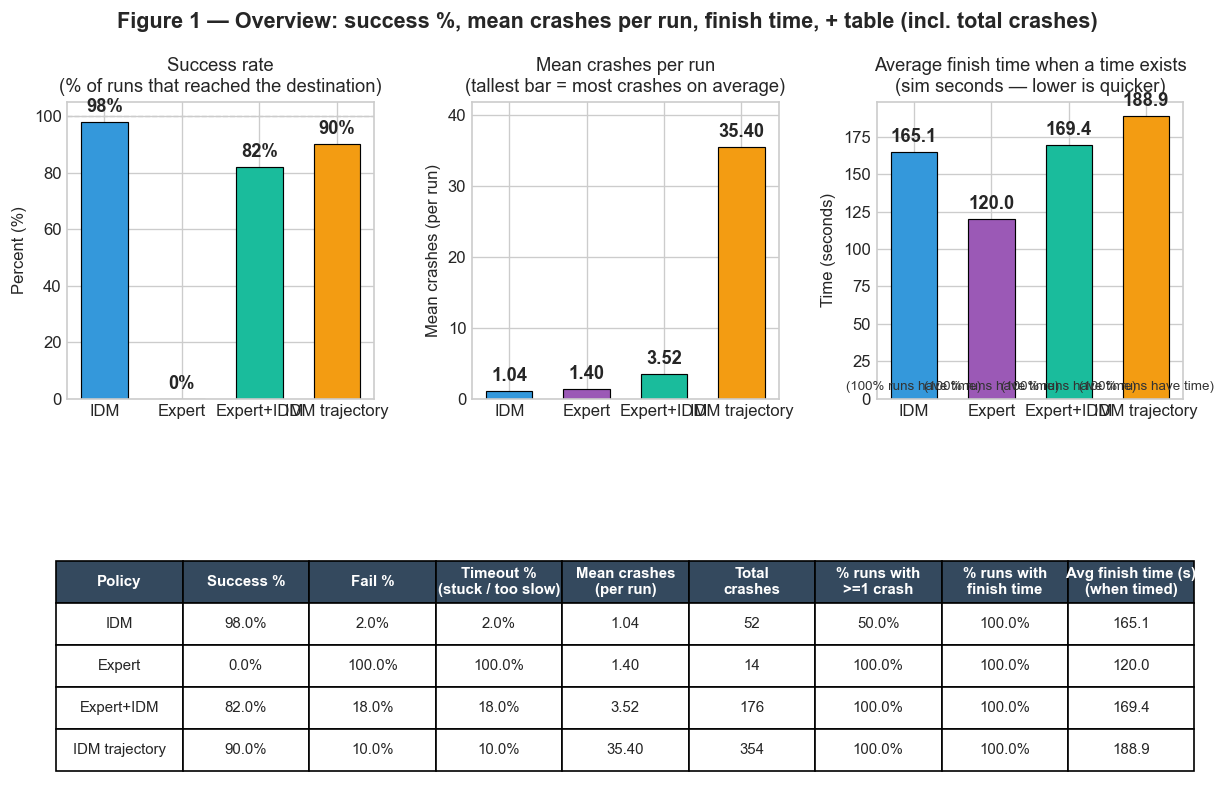
\includegraphics[width=\textwidth]{highway_policy_analysis_fig_00.png}
    \caption{Highway scenario: notebook-generated comparison of policies (first dashboard cell in \texttt{highway\_policy\_analysis.ipynb}). Bars summarise mean crashes, timeouts, and related episode statistics across all loaded workbooks.}
    \label{fig:highway_nb_0}
\end{figure}

\begin{figure}[H]
    \centering
    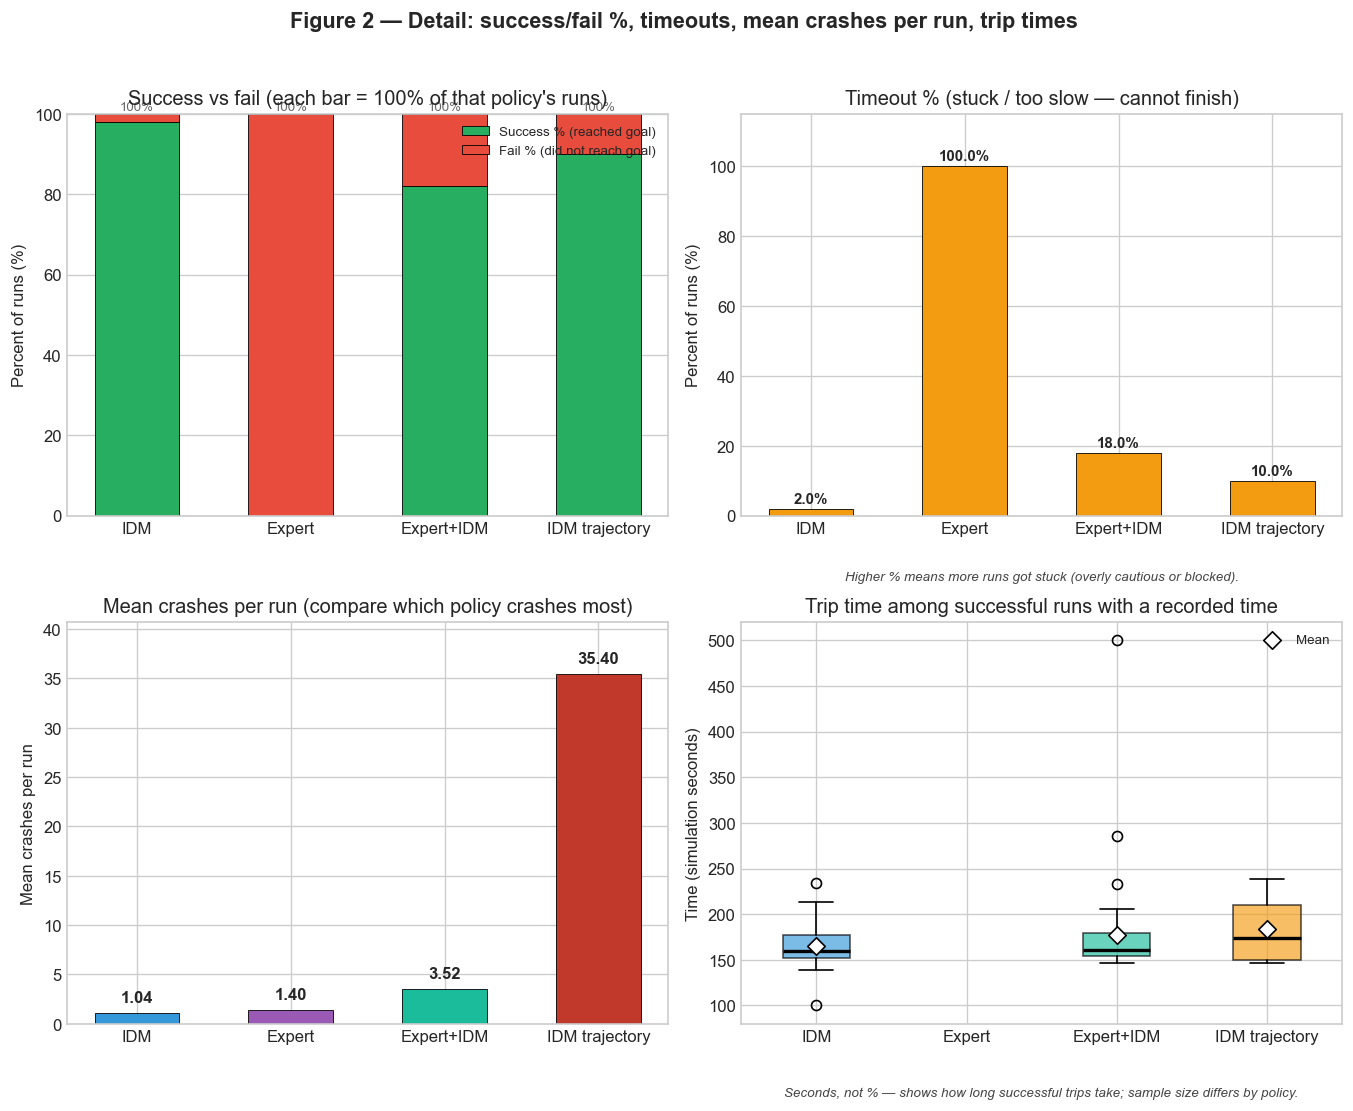
\includegraphics[width=\textwidth]{highway_policy_analysis_fig_01.png}
    \caption{Highway scenario: secondary notebook view (stacked success versus failure, timeout emphasis, and crash ranking). Interpreting these plots together with Table~\ref{tab:highway_results} prevents a single headline metric from hiding collision-heavy behaviour.}
    \label{fig:highway_nb_1}
\end{figure}

\begin{figure}[H]
    \centering
    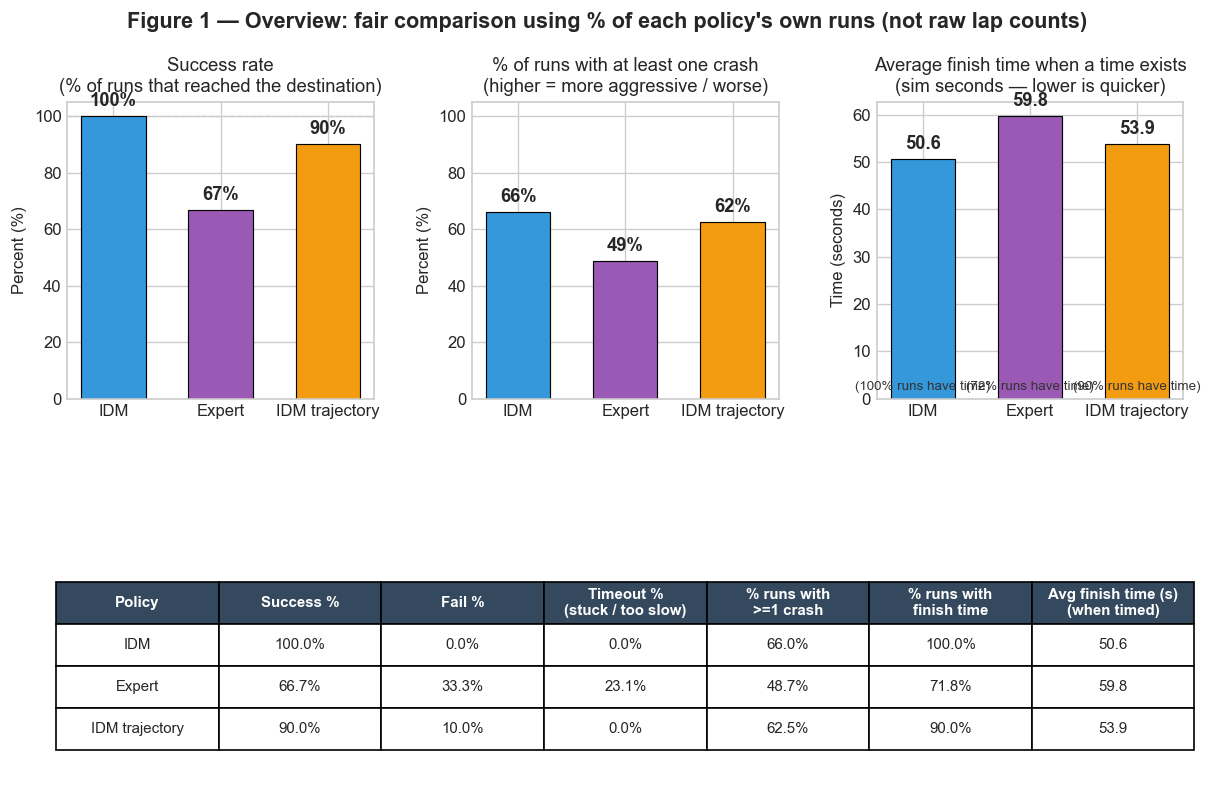
\includegraphics[width=\textwidth]{intersection_policy_analysis_fig_00.png}
    \caption{Intersection--roundabout scenario: policy comparison from \texttt{intersection\_policy\_analysis.ipynb} (first figure cell).}
    \label{fig:intersection_nb_0}
\end{figure}

\begin{figure}[H]
    \centering
    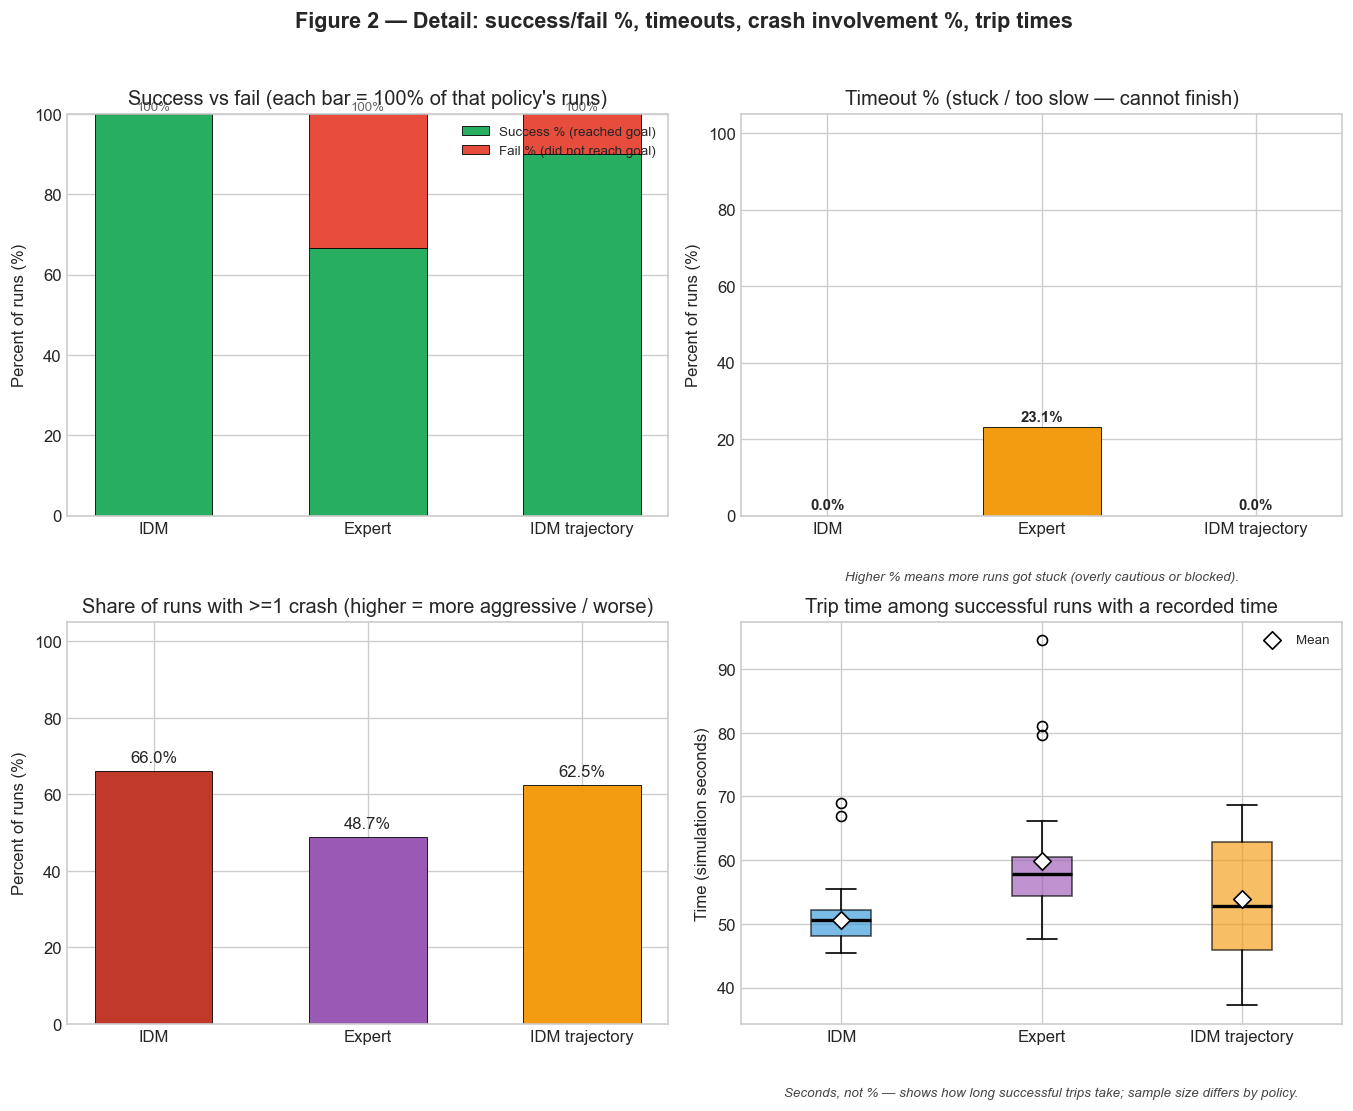
\includegraphics[width=\textwidth]{intersection_policy_analysis_fig_01.png}
    \caption{Intersection--roundabout scenario: complementary notebook breakdown (success shares, timeouts, crashes).}
    \label{fig:intersection_nb_1}
\end{figure}

\section{Highway Scenario Results}
The highway scenario produces the clearest separation between policies. IDM is the strongest overall highway policy. It completes forty-nine out of fifty episodes successfully, produces only one timeout, maintains the lowest average crash count among the strong-performing highway controllers, and shows stable average speed. This indicates that reactive control is highly effective in the tested highway environment.

Pure \texttt{ExpertPolicy} performs very poorly in this scenario. The saved results show zero successful passes across ten episodes and a timeout rate of one hundred percent. Its average speed is also much lower than the other policies. This indicates that the Expert controller, in its unmodified form, is not suitable for the tested highway configuration.

The highway-specific hybrid Expert+IDM controller improves substantially over pure Expert. It recovers many runs that would otherwise fail by switching to IDM when the ego vehicle becomes stuck. However, it still does not match plain IDM in pass rate, timeout rate, crash count, or average speed.

The trajectory-based highway controller produces a relatively high completion rate, but its crash count is extremely high. This makes it unsuitable from a safety perspective even though it often reaches the goal.

\section{Highway Policy Discussion}
The highway results can be explained by the design of both the environment and the controllers. The highway environment contains not only moving traffic, but also accident-related obstacles and static traffic objects. This means that the ego vehicle must continue making progress while reacting safely to lane-level disruption and obstruction.

IDM performs well because it is inherently reactive. It adjusts speed in response to surrounding traffic and maintains reasonably stable progress even when the route becomes partially obstructed. This makes it well matched to a highway environment that demands continuous traffic-aware adaptation.

ExpertPolicy appears to struggle because it does not recover effectively once the vehicle becomes blocked or slowed in this scenario. The custom \texttt{StuckAwareExpertPolicy} (Listing~\ref{lst:stuckaware}) exists precisely to mitigate that failure mode by handing over to IDM when speed collapses or displacement stalls. The fact that Expert+IDM still underperforms plain IDM (Table~\ref{tab:highway_results} and Figures~\ref{fig:highway_nb_0}--\ref{fig:highway_nb_1}) shows that the bottleneck is not only ``detecting'' stuck states but also the long stretches where Expert remains active and accumulates risk before the trigger fires.

The trajectory variant completes many episodes yet reports extremely high crash counts. This is consistent with Listing~\ref{lst:trajavoid}: aggressive return to geometric tracking after a short resume window can pull the vehicle back toward the reference path while surrounding traffic is still overlapping, whereas IDM-style avoidance can continue lateral evasion until the lane is clear.

\section{Intersection Scenario Results}
The intersection-roundabout scenario produces a different balance of outcomes, but IDM remains the strongest overall policy. It completes all recorded episodes successfully, avoids timeouts entirely, and maintains strong movement quality with acceptable crash performance.

ExpertPolicy performs better in the intersection scenario than in the highway scenario. It achieves some successful runs and produces the lowest average crash count among the tested policies. However, its pass rate remains low and its average speed is also much lower than the other methods.

TrajectoryIDM is more competitive in the intersection scenario than in the highway scenario. It achieves a higher pass rate than Expert and the highest average speed among the three policies. However, it also records the highest crash count.

\section{Intersection Policy Discussion}
The intersection-roundabout environment differs from the highway case because the route is shorter, more constrained, and built around explicit conflict points. The target vehicle must follow a fixed path while timing its movements relative to other agents entering or occupying the same junction areas.

This structure appears to help ExpertPolicy compared with the highway case. However, the low pass rate still shows that cautious behaviour alone is not sufficient. A useful policy must also complete the route reliably.

TrajectoryIDM is better suited to this environment because the fixed route can be represented clearly as a geometric path (Chapter~5). However, the higher crash frequency in Table~\ref{tab:intersection_results} and Figures~\ref{fig:intersection_nb_0}--\ref{fig:intersection_nb_1} shows that route adherence and movement efficiency can come at the cost of more aggressive interaction with surrounding vehicles. IDM avoids this trade-off most successfully here because every agent uses the same reactive law, reducing inconsistent predictions between agents.

\section{Street Scenario Results}
The street scenario must be interpreted more cautiously because the saved results are less complete than those for the highway and intersection scenarios. The strongest street result set is the ten-episode Expert workbook, in which ExpertPolicy completes all episodes successfully with zero crashes and zero timeouts.

The available IDM street results are fewer in number, but they also show clean behaviour with no recorded crashes and no timeouts. This suggests that IDM is also capable of handling the street scenario effectively under the available test conditions.

\begin{figure}[H]
    \centering
    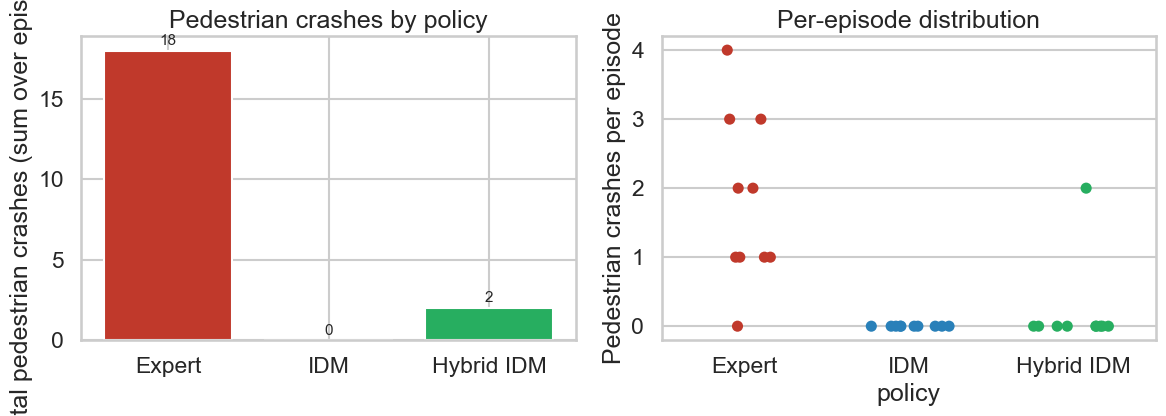
\includegraphics[width=\textwidth]{street_policy_comparison_fig_00.png}
    \caption{Street scenario: visualization from \texttt{street\_policy\_comparison\_visualization.ipynb} (supports Table~\ref{tab:street_results}; sample sizes differ).}
    \label{fig:street_nb_0}
\end{figure}

\section{Street Policy Discussion}
The street environment appears to match ExpertPolicy better than the other two scenarios. One reason is that the route is narrower and more deterministic, while the pedestrian event, although dynamic, is still triggered in a controlled way according to route progress and approach conditions. This makes the environment challenging without creating the same obstacle-heavy instability seen in the highway case.

The available IDM street outputs also indicate stable performance, but the dataset is currently smaller. For that reason, the correct interpretation is not that one policy has been fully proven superior in the street case, but that both policies perform well in the available saved outputs.

\section{Cross-Scenario Comparison}
A cross-scenario comparison reveals the main contribution of the project. Policy quality is strongly environment-dependent. A controller that performs well in one scenario can become weak in another when the road structure, traffic behaviour, or event complexity changes.

IDM is the most reliable all-round policy in the project. It performs best overall in the highway and intersection scenarios and also shows clean behaviour in the available street records. ExpertPolicy is highly scenario-sensitive. TrajectoryIDM is most useful when route geometry is explicit and stable, as in the intersection-roundabout task, but becomes less suitable when stronger reactive obstacle handling is needed.

\section{Main Findings}
\begin{enumerate}[label=\arabic*.]
    \item Plain IDM is the strongest overall policy across the recorded highway and intersection experiments.
    \item Pure ExpertPolicy is not suitable for the tested highway environment.
    \item Adding IDM fallback improves Expert performance on the highway, but still does not make it better than plain IDM.
    \item Trajectory-guided control can be useful in route-structured environments, but may become unsafe when strong reactive obstacle handling is required.
    \item The street scenario is the strongest recorded environment for ExpertPolicy, with the complete ten-episode run showing perfect completion and zero crashes.
    \item The custom scenario implementations are sufficient to expose meaningful differences between policy types.
    \end{enumerate}

\chapter{Conclusion and Future Work}

\section{Conclusion}
This project developed a complete simulation-based framework for evaluating autonomous driving policies in MetaDrive across three scenario categories: highway, intersection-roundabout, and street. The work combined custom environment implementation, built-in MetaDrive policy comparison, scenario-specific control extensions, repeated episode testing, structured result export, and workbook-based analysis.

The results show clearly that autonomous driving policy performance is strongly dependent on scenario type. IDM delivers the strongest overall performance in the highway and intersection environments, offering the best balance between completion, stability, and safety. ExpertPolicy performs poorly in the tested highway scenario, achieves mixed results in the intersection scenario, and performs strongly in the street scenario. TrajectoryIDM demonstrates that explicit route-following can be beneficial in route-structured tasks, but also shows that high completion is not sufficient if crash frequency becomes too high.

The project therefore succeeds in its central objective: it provides a practical and evidence-based framework for comparing autonomous driving policies across multiple MetaDrive scenarios. More importantly, it shows that policy suitability must be interpreted relative to the environment in which the controller operates.

\section{Limitations of the Current Project}
Although the project produces useful findings, it also has several limitations. First, the work is entirely simulation-based and does not include real vehicles, real sensors, or real-world deployment. Second, the number of saved runs is not identical across all policy-scenario combinations. Third, the compared controllers are limited mainly to built-in MetaDrive policies and scenario-specific modifications rather than learning-based policies or advanced planning systems. Fourth, the conclusions are tied to the specific road layouts, traffic settings, and event conditions implemented in the project scripts.

\section{Future Work}
Several directions for future work can extend this project meaningfully. One immediate improvement would be to increase the number of saved street episodes, especially for IDM, so that the street comparison is supported by a dataset as strong as the highway and intersection datasets. Another useful direction would be to expand the scenario library to include denser urban routes, more complex intersections, larger pedestrian populations, or additional edge-case traffic situations.

The policy set could also be extended. Since the current framework already supports structured scenario comparison and metric logging, it would be suitable for evaluating reinforcement learning agents, more advanced planning-based controllers, or additional hybrid control strategies against the current MetaDrive baselines.

Future work could also improve the analysis pipeline by adding automated statistical testing, confidence intervals, and more formal safety indicators. Finally, the project could move toward richer realism through sensor-based integration or broader closed-loop testing if the goal expands from scenario-based policy comparison to more comprehensive autonomous driving validation.

\bibliographystyle{IEEEtran}
\bibliography{references}

\appendix
\chapter{Overleaf Notes}
This directory is packaged for upload as a single Overleaf project.
\begin{enumerate}[label=\arabic*.]
    \item Upload the whole \texttt{Overleaf\_Package} folder (or a zip of it) to Overleaf via \emph{New Project} $\rightarrow$ \emph{Upload Project}.
    \item Set the main document to \texttt{main.tex} (Menu $\rightarrow$ Main document).
    \item Place your NTU logo image at \texttt{figures/ntu\_logo.png}. If the file is missing, compilation will fail on the title page until you add it.
    \item \texttt{references.bib} must sit next to \texttt{main.tex}; figures must stay under \texttt{figures/} because \verb|\graphicspath{{figures/}}| is set in the preamble.
    \item Compiler: \texttt{pdfLaTeX}. Overleaf runs \texttt{bibtex} automatically; the \texttt{IEEEtran} bibliography style is available in the default TeX Live image.
\end{enumerate}

\end{document}
